\chapter{THE STANDARD MODEL AND SUPERSYMMETRY}
\label{chap:theory}

\section{The standard model of particle physics}
\label{sec:StandardModel}
The standard model (SM) of particle physics is a non-Abelian gauge theory that describes elementary particles and their allowed interactions
The first piece of the standard model was developed in 1961 (XX references! XX) with the unification of the electromagnetic and weak interactions. 
The Higgs mechanism was later incorporated into the standard model in 1967 (XX cite XX), and 
the standard model took on the form we know today with the inclusion of the strong force and quantum chromodynamics (QCD) in the 1970's (XX cite XX).
The standard model is incredibly successful, and it has made absurdly precise predictions that have held up to experimental scrutiny. 

The standard model is a Lorentz-invariant quantum field theory. The symmetry group of the standard model is 
\begin{equation}
G_{SM} = SU(3)_C \otimes SU(2)_L \otimes SU(1)_\Upsilon
\label{equ:symm}
\end{equation}
where $SU(3)_C$ is responsible for mixing the 3 \textit{colors} of quarks and antiquarks, $SU(2)_L$ represents \textit{weak isospin}, and $U(1)_\Upsilon$ couples to the \textit{weak hypercharge $\Upsilon$}. The combination $SU(2)_L \otimes SU(1)_\Upsilon$ corresponds to the electroweak interactions. 

%%%%%%%%%%%%%%%%%%%%%%%%%%%%%%%%%%%%%%%

The fields in the SM are identified by their representation in the symmetry group of Equation~\ref{equ:symm}. These are listed for the SM fermions in Table~\ref{tab:fermions} and for the gauge bosons in Table~\ref{tab:bosons}. There are three generations of quarks and three generations of leptons in the SM. The quarks are in a non-trivial representation of all three SM symmetries, and therefore interact via the strong, weak, and electromagnetic interactions. The three ``up-type" quarks are the up quark $u$, the charm quark $c$, and the top quark $t$. The three ``down-type" quarks are the down quark $d$, the strange quark $s$, and the bottom quark $b$. 

The three generations of leptons include the electron $e$, muon $\mu$, and tau $\tau$ and the corresponding neutrinos. In the SM, the neutrinos are massless, even though it has been experimentally established that at least two of the neutrinos must have non-zero mass XX citeXX. The electron, muon and tau particles participate in the weak interaction and the electromagnetic interaction, but the neutrinos, being electromagnetically neutral, only participate in the weak interaction. 

\begin{table}[ht]
    \caption{FERMIONS IN THE STANDARD MODEL}
    \centering
    \begin{tabular}{|c|c|c|c|}
    \hline
    \hline
    Name  & Symbol & $SU(3)_C,~SU(2)_L,~U(1)_\Upsilon $\\
  	  \hline
           \hline    
quarks        & ($u_L~d_L$)     & (\textbf{3}, \textbf{2}, $\frac{1}{6}$) \\
(3 families) & $u_R^\dagger$ & ($\bar{\textbf{3}}$, \textbf{1}, $-\frac{2}{3}$) \\
                   & $d_R^\dagger$ & ($\bar{\textbf{3}}$, \textbf{1}, $\frac{1}{3}$) \\
                   \hline
leptons       & ($\nu~e_L$)      &  (\textbf{1}, \textbf{2}, $-\frac{1}{2}$) \\
(3 families) & $e_R^\dagger$ &  (\textbf{1}, \textbf{1}, 1) \\
           \hline
           \hline
    \end{tabular}
    \label{tab:fermions}
%    \justify{Fermions in the standard model. }
\end{table}

%%%%%%%%%%%%%%%%%%%%%%%%%%%%%%%%%%%%%%%

The gauge bosons are responsible for mediating the interactions between the fermions. Before electroweak symmetry breaking (EWSB), the three gauge bosons of $SU(2)_L$ are the $W^+,~W^-,$ and $W^0$, and the $U(1)_\Upsilon$ gauge boson is the $B$ boson. After EWSB, the $W^+$ and $W^-$ bosons gain a mass, and the $W_0$ and $B$ bosons mix to form the massive $Z$ boson and the massless photon $\gamma$. EWSB will be described in more detail in Section~\ref{sec:EWSB}.

For the strong force $SU(3)_C$, the gauge bosons are the gluons. Processes involving the interactions of quarks and gluons are referred to as QCD processes. The QCD interaction is different from the electroweak interactions in that the strong force grows in strength at larger distances. This leads to the phenomenon of \textit{confinement}: at low energies and large distances (greater than ~1 GeV$^-1$), we cannot identify individual quarks or gluons. Instead, these particles can only be found in $SU(3)_C$ singlets, typically either mesons ($q\bar{q}$) or baryons ($qqq$ or $\bar{q}\bar{q}\bar{q}$). 

\begin{table}[ht]
    \caption{GAUGE BOSONS IN THE STANDARD MODEL}
    \centering
    \begin{tabular}{|c|c|c|c|}
    \hline
    \hline
    Name  & Symbol & $SU(3)_C,~SU(2)_L,~U(1)_\Upsilon $\\
  	  \hline
           \hline    
gluon         & $g$   & (\textbf{8}, \textbf{1}, 0) \\
\hline
$W$ bosons & $W^\pm,~W^0$ & (\textbf{1}, \textbf{3}, 0) \\
\hline
$B$ boson & $B^0$ & (\textbf{1}, \textbf{1}, 0) \\
           \hline
           \hline
    \end{tabular}
    \label{tab:bosons}
    \justify{Gauge bosons in the standard model before electroweak symmetry breaking. }
\end{table}

%%%%%%%%%%%%%%%%%%%%%%%%%%%%%%%%%%%%%%%

Finally, the only particle not included in Table~\ref{tab:fermions} or \ref{tab:bosons} is the Higgs boson. The Higgs boson was discovered by the CMS and ATLAS collaborations in 2012 XX cite XX, and is responsible for electroweak symmetry breaking (EWSB), which will be described in Section~\ref{sec:EWSB}. It is the only fundamental scalar in the SM and has a mass of approximately 125 GeV. The Higgs boson is in the  (\textbf{1}, \textbf{2}, $+\frac{1}{2}$) representation of $G_{SM}$, and is therefore uncharged under the strong and electromagnetic interactions. 

Figure~\ref{fig:SMint} summarizes the SM particles and their allowed interactions.

\begin{figure*}[htbp]
    \centering
    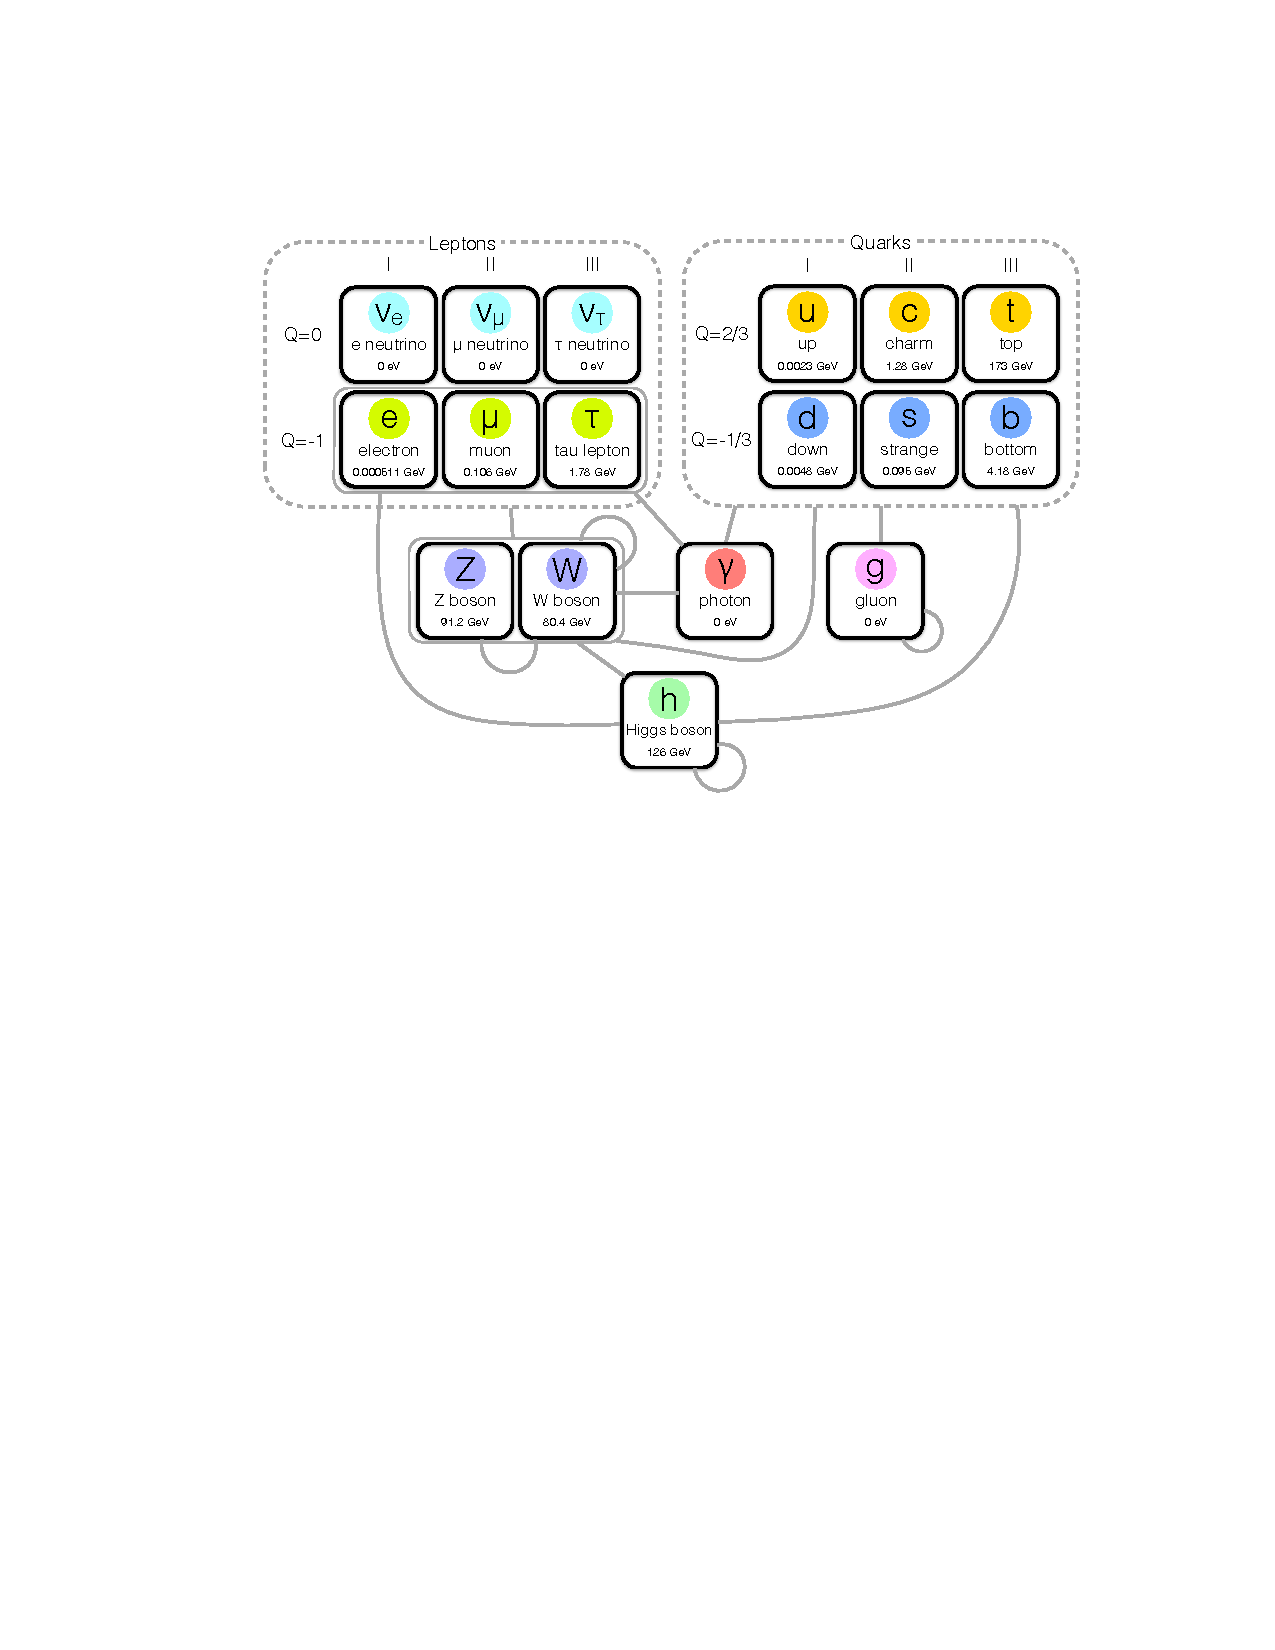
\includegraphics[width=\textwidth]{Figures/Theory/SM_Interactions.pdf}
    \caption{Particle content of the standard model. Allowed interactions are indicated with gray lines between particles or particle groups. The mass of each particle is listed underneath its symbol and name. The electric charge Q of the leptons and quarks is also indicated. Particles connected to themselves can have self-interactions.
    Reprinted from Reference~\cite{Yutaro}.}
    \label{fig:SMint}
\end{figure*}

%%%%%%%%%%%%%%%%%%%%%%%%%%%%%%%%%%%%%%%
%%%%%%%%%%%%%%%%%%%%%%%%%%%%%%%%%%%%%%%

\subsection{Electroweak symmetry breaking}
\label{sec:EWSB}
The electroweak symmetry is spontaneously broken by the non-zero vacuum expectation value (vev) of the Higgs. After spontaneous symmetry breaking (SSB), the remaining symmetry is $U(1)_{\textrm{EM}}$, which corresponds to the electromagnetic interaction. After electroweak symmetry breaking, there are three massive gauge bosons---the $W-^\pm$ and $Z$ bosons---and the massless photon $\gamma$.  The photon couples to the electric charge q: 
\begin{equation}
q = T^3 + \Upsilon
\end{equation}
where $\Upsilon$ is the weak hypercharge and $T^3$ is the isospin.

%%%%%%%%%%%%%%%%%%%%%%%%%%%%%%%%%%%%%%%
\subsection{Limitations of the standard model}
\label{sec:SMweakness}


%%%%%%%%%%%%%%%%%%%%%%%%%%%%%%%%%%%%%%%

Weak interactions only occur over short ranges because $W-^\pm$ and $Z$ are massive.

particle content: three generations of leptons and quarks
plot showing how the particles interact
Bosons mediate the interactions

12 vector fields (spin 1)- gauge fields of the SU(3) x SU(2) x U(1)
45 Weyl fermion fields: [21 Dirac spinors  (3 colors x 6 quarks) + 3 charged leptons] x2 to get to  weyl+ 3 neutrinos
complex doublet H of scalar fields

Left-handed Weyl components of quark Dirac spinors form 9 doublets of $SU(2)_W$ (3 flavor doublets per 3 color)
Right-handed Weyl components of quark Dirac spinors are 18 $SU(2)_W$ singlets. Weak interactions can break parity

Left-handed leptons form 3 $SU(2)_W$ doublets 
right-handed leptons form singlets. If right-handed neutrinos exist, they are sterile and we have no evidence (can't have evidence?) for them
Dirac spinor $\Psi$ and conjugate $\bar{\Psi}$ are equivalent to two left-handed Weyl spinors ($\chi$ and $\tilde{\chi}$)
and their right-handed conjugates ($\chi^\dagger$ and $\tilde{\chi}^\dagger$).Tilde = anti


%http://bolvan.ph.utexas.edu/~vadim/Classes/2011f/SM.pdf

\section{Supersymmetry}
\label{sec:SUSY}

Motivations:
Higgs mass, contributions 
Hierarchy problem 

\begin{table}[ht]
    \caption{CHIRAL SUPERMULTIPLETS IN MSSM}
    \centering
    \begin{tabular}{|c|c|c|c|c|}
    \hline
    \hline
    \multicolumn{2}{|c|}{Names} & Spin 0 & Spin 1/2 &$SU(3)_C,~SU(2)_L,~U(1)_\Upsilon $\\
  	  \hline
           \hline    
squarks, quarks  & Q & ($\tilde{u}_L~\tilde{d}_L$) & ($u_L~d_L$)  & (\textbf{3}, \textbf{2}, $\frac{1}{6}$) \\
(3 families) & $\bar{u}$ & $\tilde{u}_R^\ast$ & $u_R^\dagger$ & ($\bar{\textbf{3}}$, \textbf{1}, $-\frac{2}{3}$) \\
                   & $\bar{d}$ & $\tilde{d}_R^*$     & $d_R^\dagger$ & ($\bar{\textbf{3}}$, \textbf{1}, $\frac{1}{3}$) \\
                   \hline
sleptons, leptons  & $L$ & ($\tilde{\nu}~\tilde{e}_L$) & ($\nu~e_L$)      &  (\textbf{1}, \textbf{2}, $-\frac{1}{2}$) \\
(3 families) & $\bar{e}$ & $\tilde{e}_R^\ast$  & $e_R^\dagger$ &  (\textbf{1}, \textbf{1}, 1) \\
\hline
Higgs, higgsinos & $H_u$  & ($H_u^+ ~ H_u^0$) & ($\tilde{H}_u^+ ~ \tilde{H}_u^0$) & ($\textbf{1}$, \textbf{2}, $+\frac{1}{2}$) \\
                           & $H_d$  & ($H_d^0 ~ H_d^-$) & ($\tilde{H}_d^0 ~ \tilde{H}_d^-$) & ($\textbf{1}$, \textbf{2}, $-\frac{1}{2}$) \\
           \hline
           \hline
    \end{tabular}
    \label{tab:SUSY_fermions}
    \justify{Reprinted from Reference~\cite{SUSYprimer}.}
\end{table}

\section{Gauge-mediated supersymmetry breaking}
\label{sec:gmsb}

